%!TEX program = xelatex
% 完整编译: xelatex -> biber/bibtex -> xelatex -> xelatex
\documentclass[lang=cn,11pt,a4paper]{elegantpaper}

\title{基于Python的手势控制和交互}
\author{18-陈雨竹-PB19000160, 16-张奇-PB19000093}
\institute{USTC}

\date{\zhtoday}

\usepackage{array,verbatim,fancyhdr,amsmath,graphicx}
\usepackage{amssymb,subfig,hyperref}

\begin{document}

\maketitle
\begin{abstract}
\end{abstract}

\section{项目简介}

本项目是基于Python开发的手势交互鼠标、键盘、游戏任务交互的若干例子. 
用户可以利用摄像头, 完成虚拟键盘输入、在画板上画画、拖动滑块移动、
交互网页游戏、交互内置游戏等操作. 源代码已开源到
\href{https://github.com/cyzkrau/Gestures2Operation}
{https://github.com/cyzkrau/Gestures2Operation}

\section{编程环境和核心方法}

本文的项目需要在x86的Python上运行, 具体运行方法可见Github上的说明文档. 

本文的核心方法是在不断的利用摄像头读取单张图片, 并识别出其中手的关键点. 
利用摄像头读取单张图像可以使用OpenCV中的VideoCapture函数. 
识别单张图片中手的关键点可使用谷歌mediapipe包进行操作. 

\begin{figure}[htb]
  \centering
  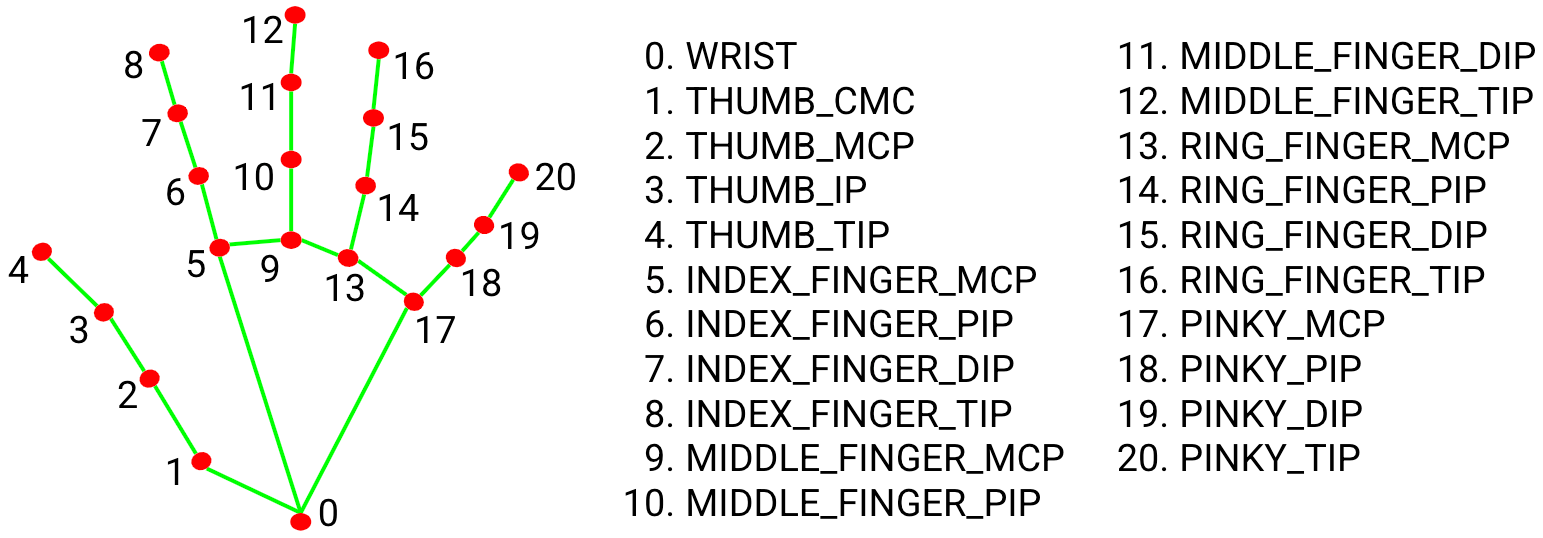
\includegraphics[width=.8\textwidth]{imgs/hand_landmarks.png}
  \caption{手21关键点\label{ldmk}}
\end{figure}

mediapipe使用锚点方法和非极大值抑制方法对手掌识别模型进行训练, 
实现了 95.7\% 的平均精度, 再用Hand Landmark Model计算出识别出的21关键点
位置, 这21关键点所代表的关节信息如图\ref{ldmk}. 

\section{项目细节}
目前基于摄像头的手势控制交互, 如图\ref{pc1}, 已经完成的样例有
虚拟键盘输入、在画板上画画、拖动滑块移动、交互网页游戏、交互内置游戏. 
其中陈雨竹负责完成画板上画画和交互网页游戏, 张奇负责完成虚拟键盘输入、
拖动滑块移动和交互内置游戏. 

\begin{figure}[htb]
  \centering
  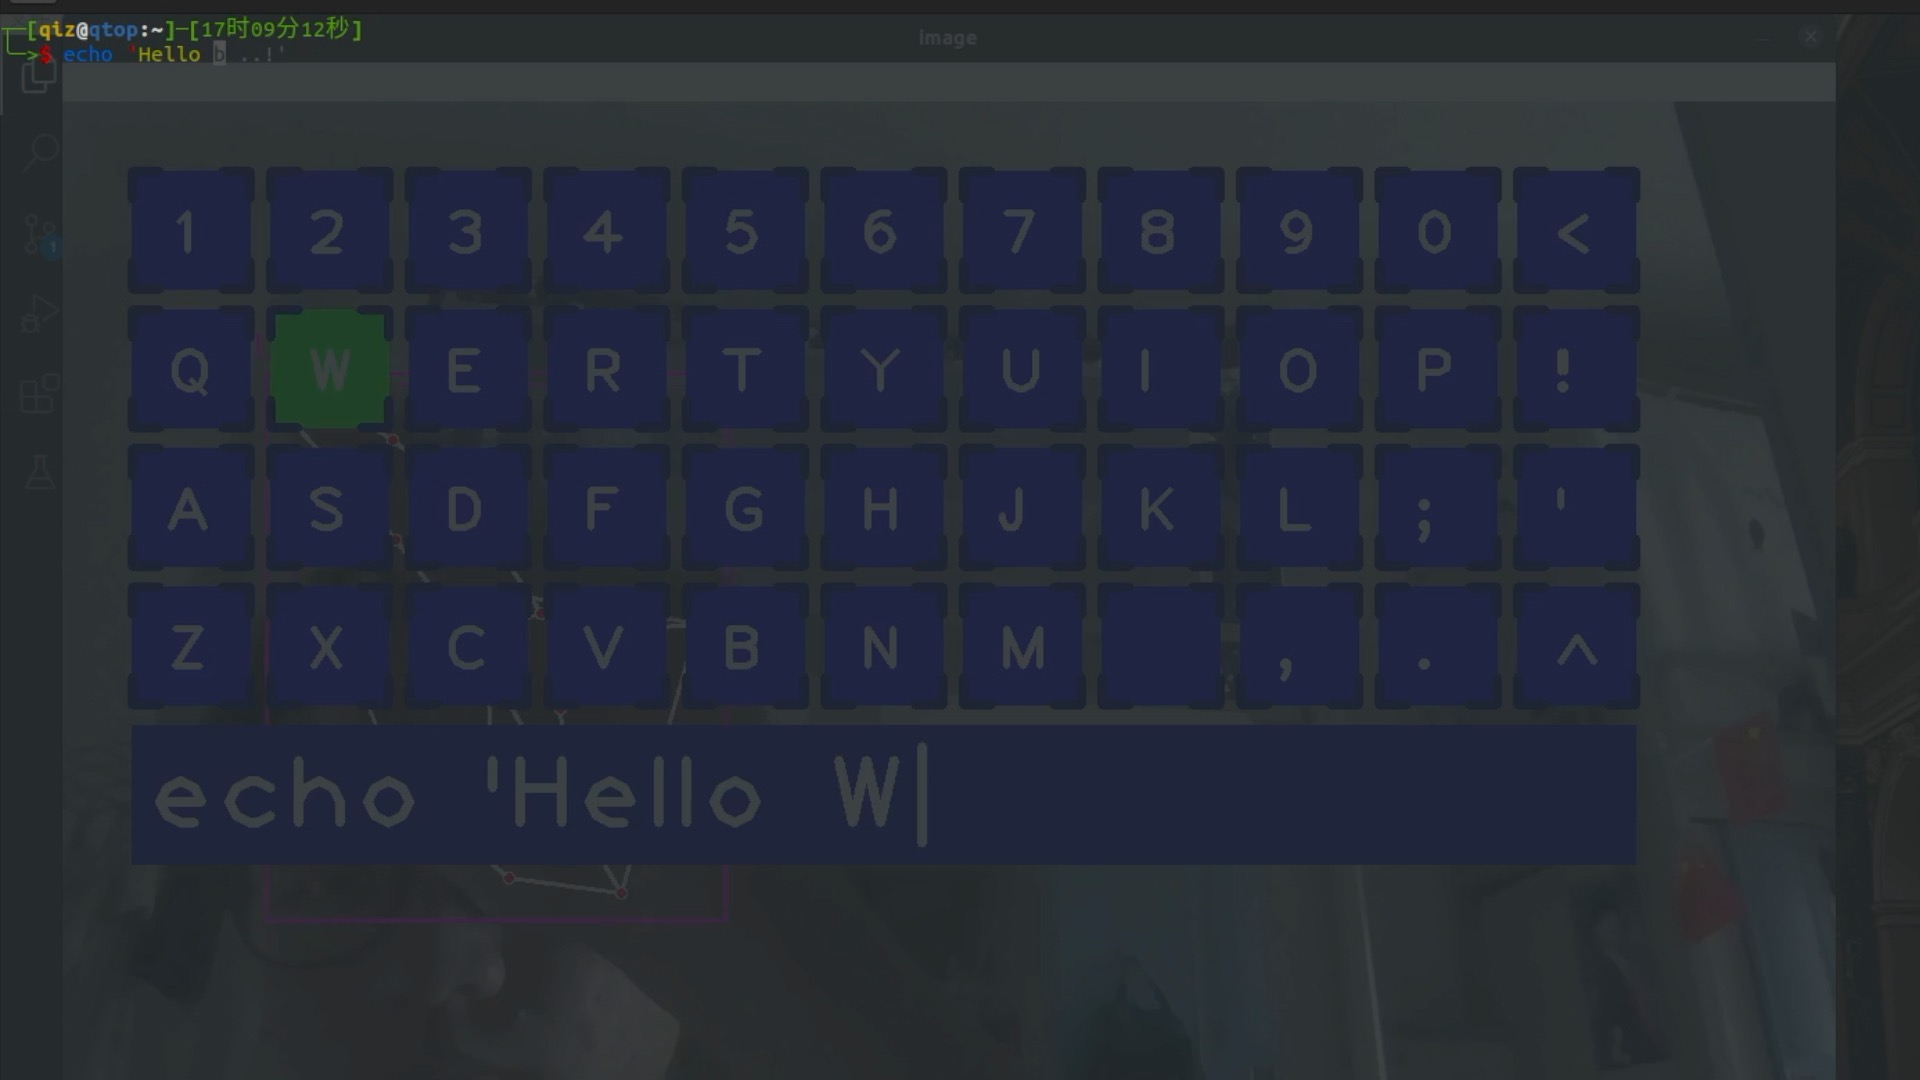
\includegraphics[width=.3\textwidth]{imgs/demo1.jpg}$\quad$
  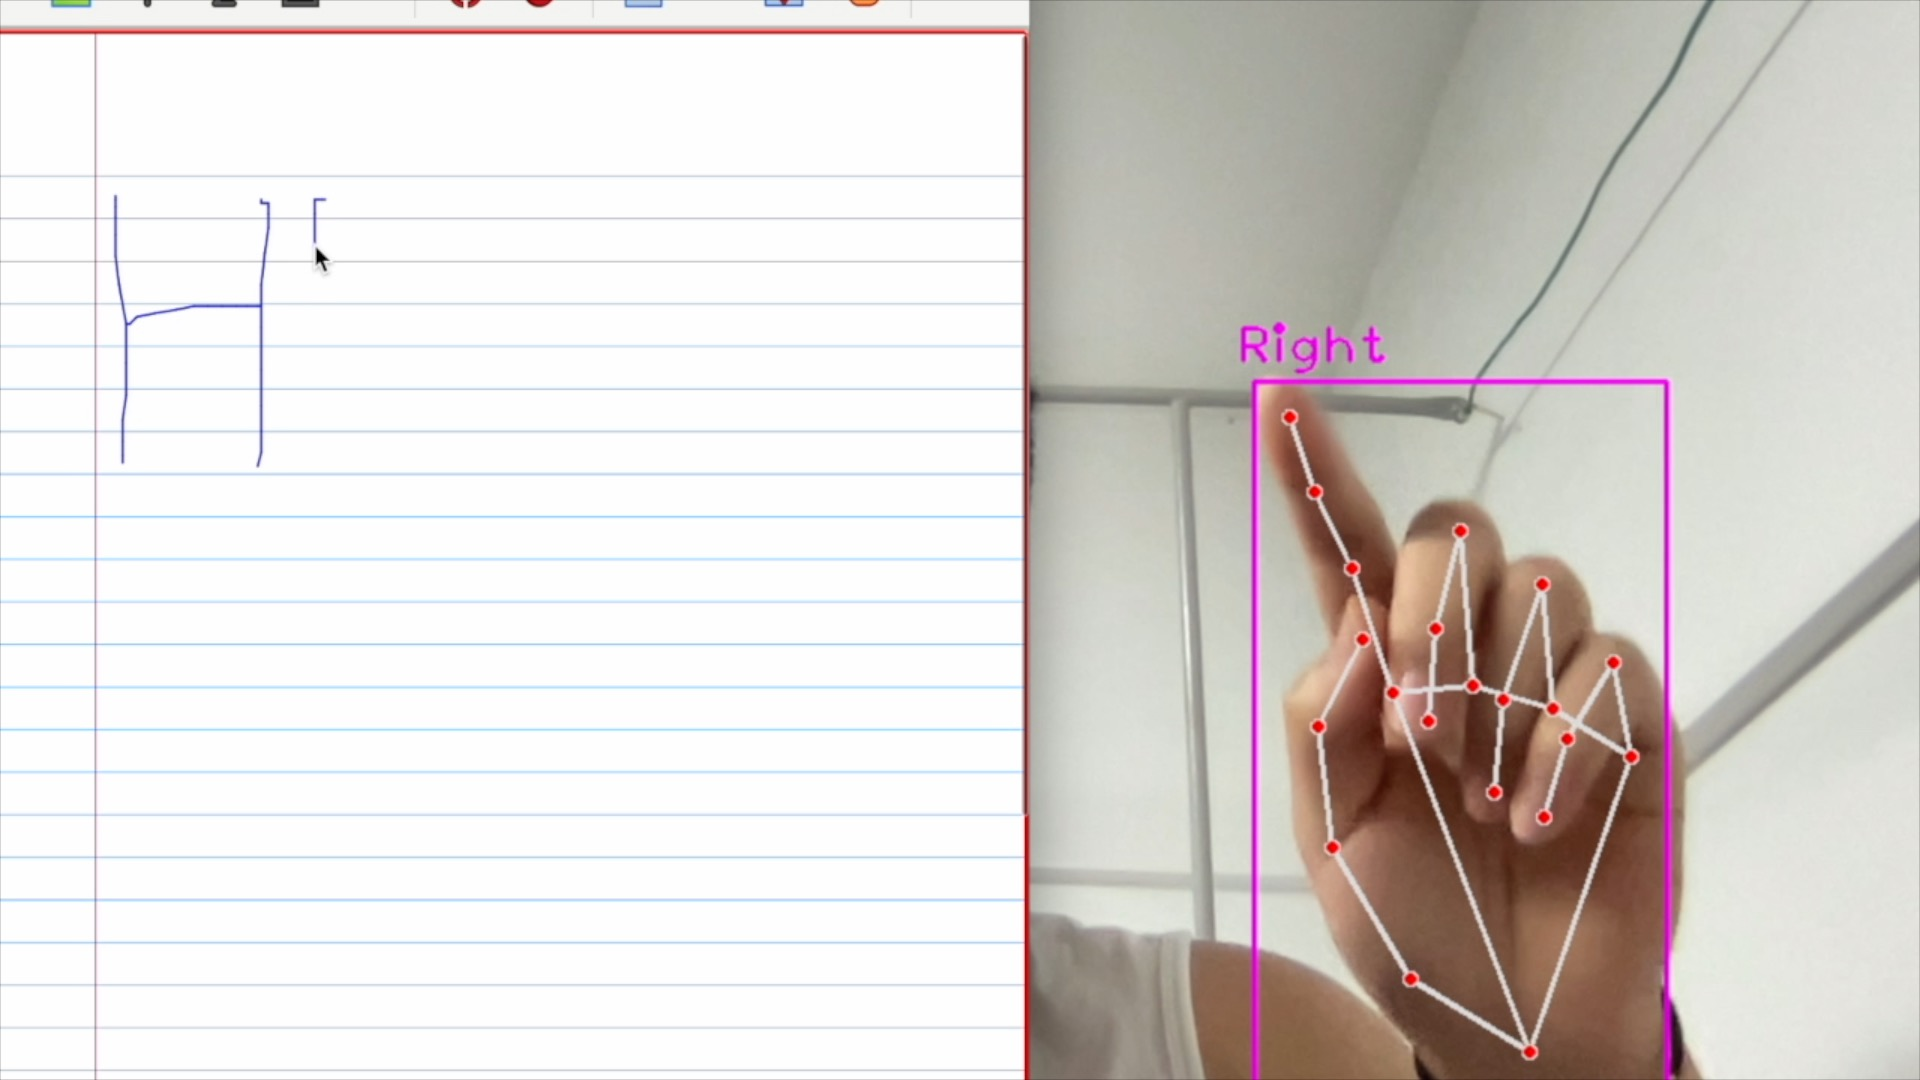
\includegraphics[width=.3\textwidth]{imgs/demo2.jpg}$\quad$
  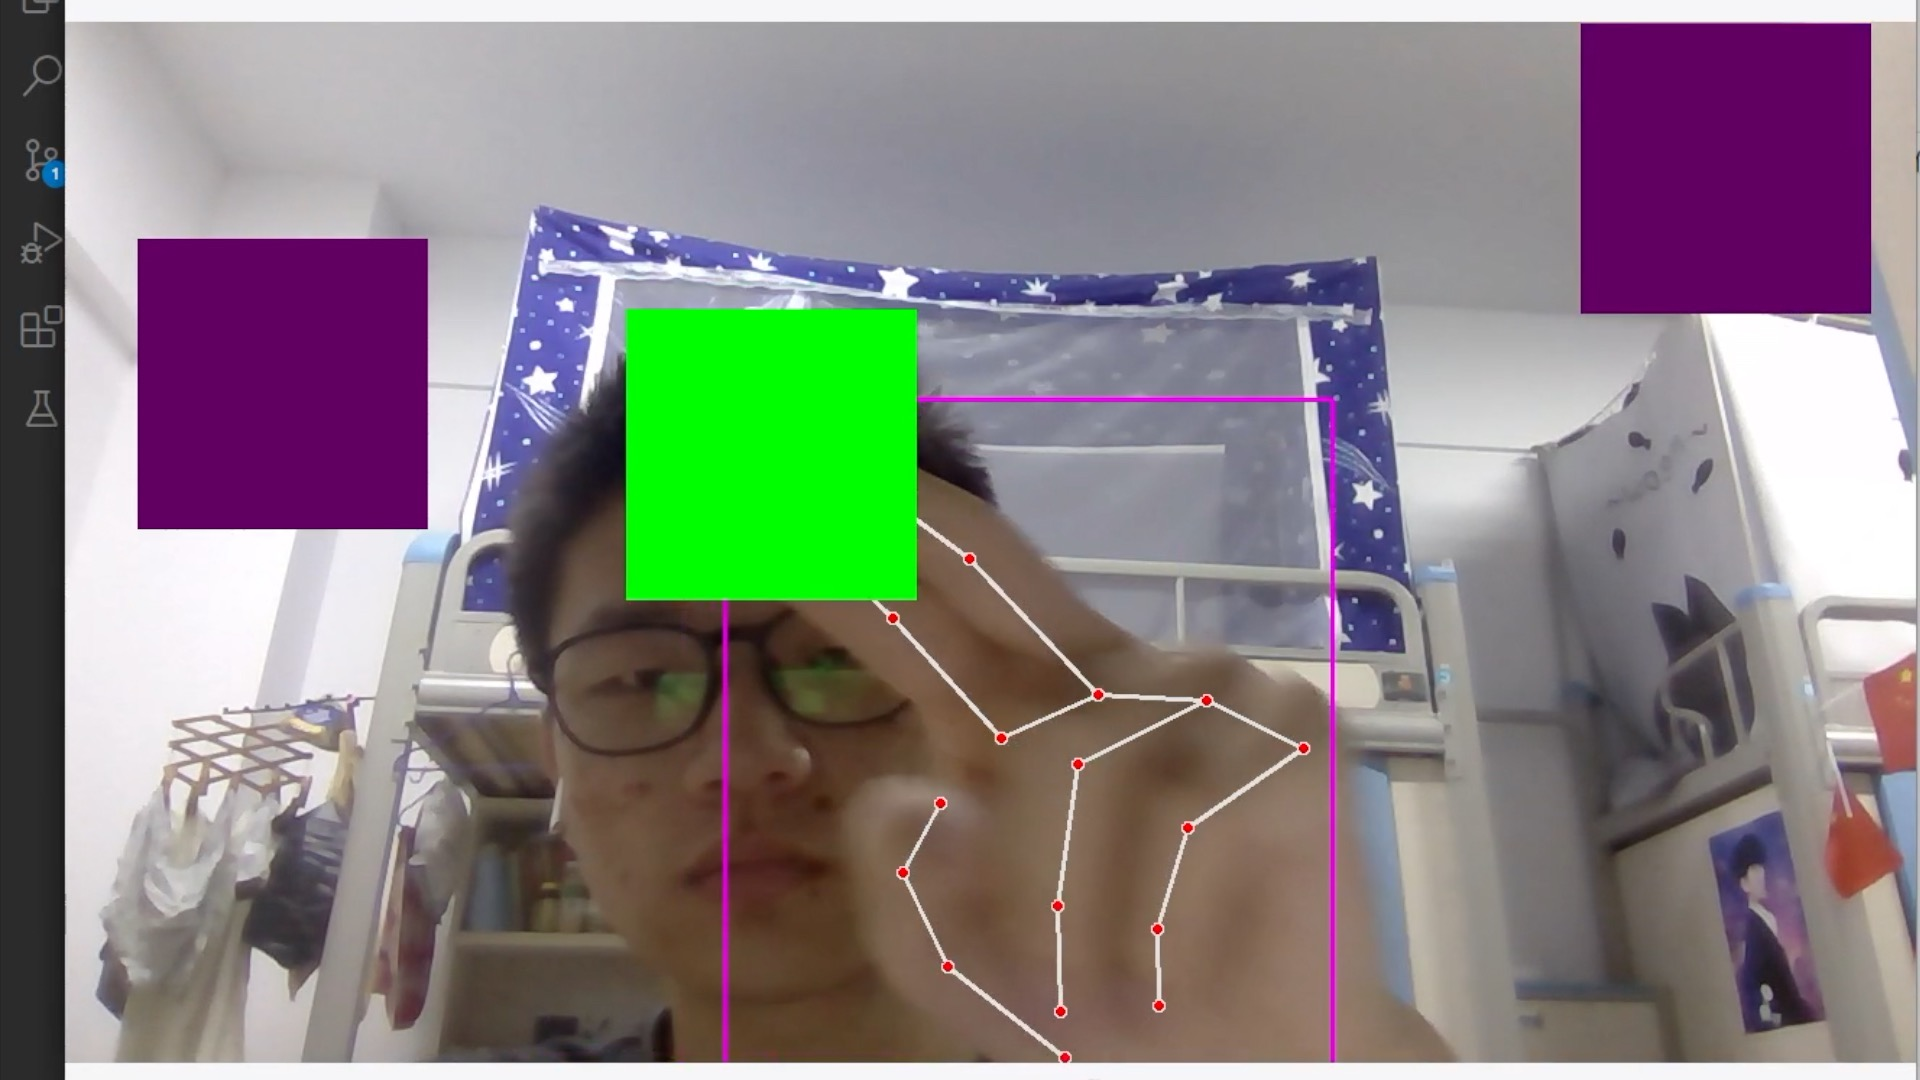
\includegraphics[width=.3\textwidth]{imgs/demo3.jpg}$\quad$
  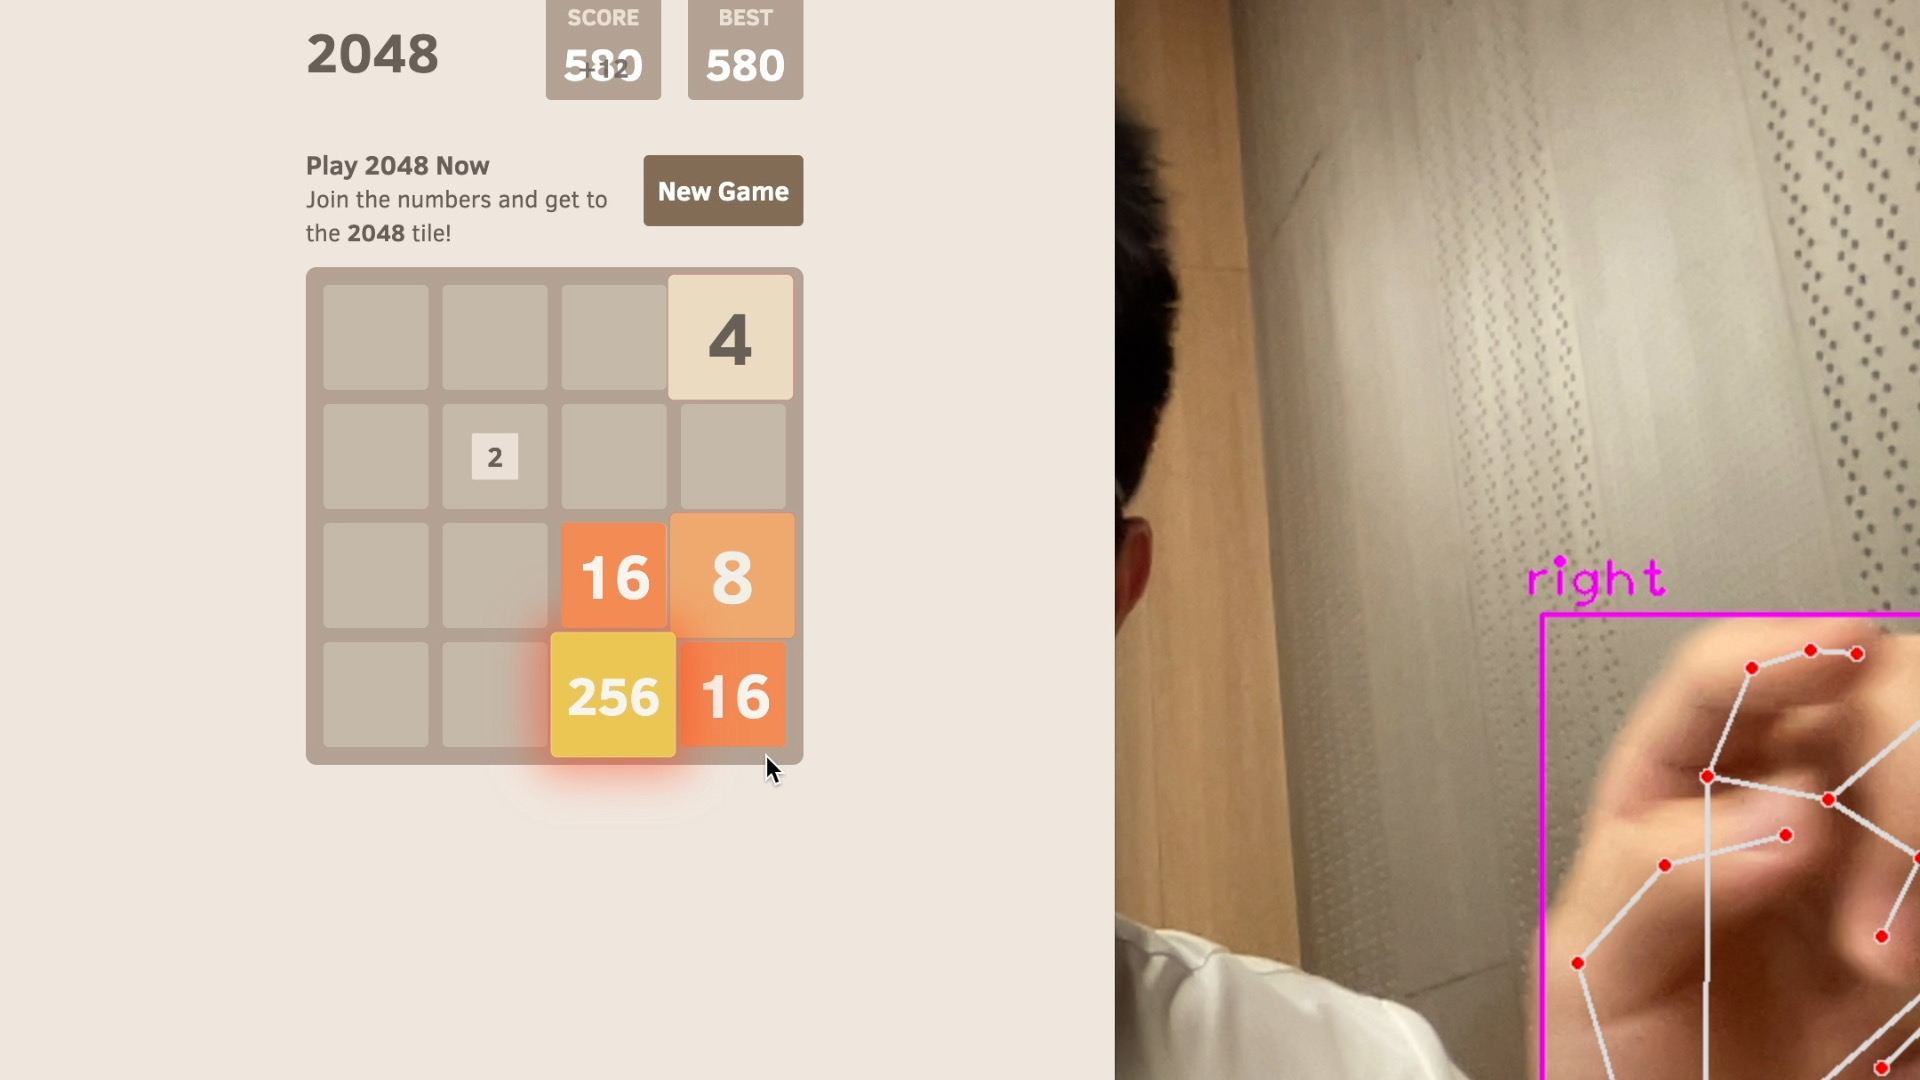
\includegraphics[width=.3\textwidth]{imgs/demo4.jpg}$\quad$
  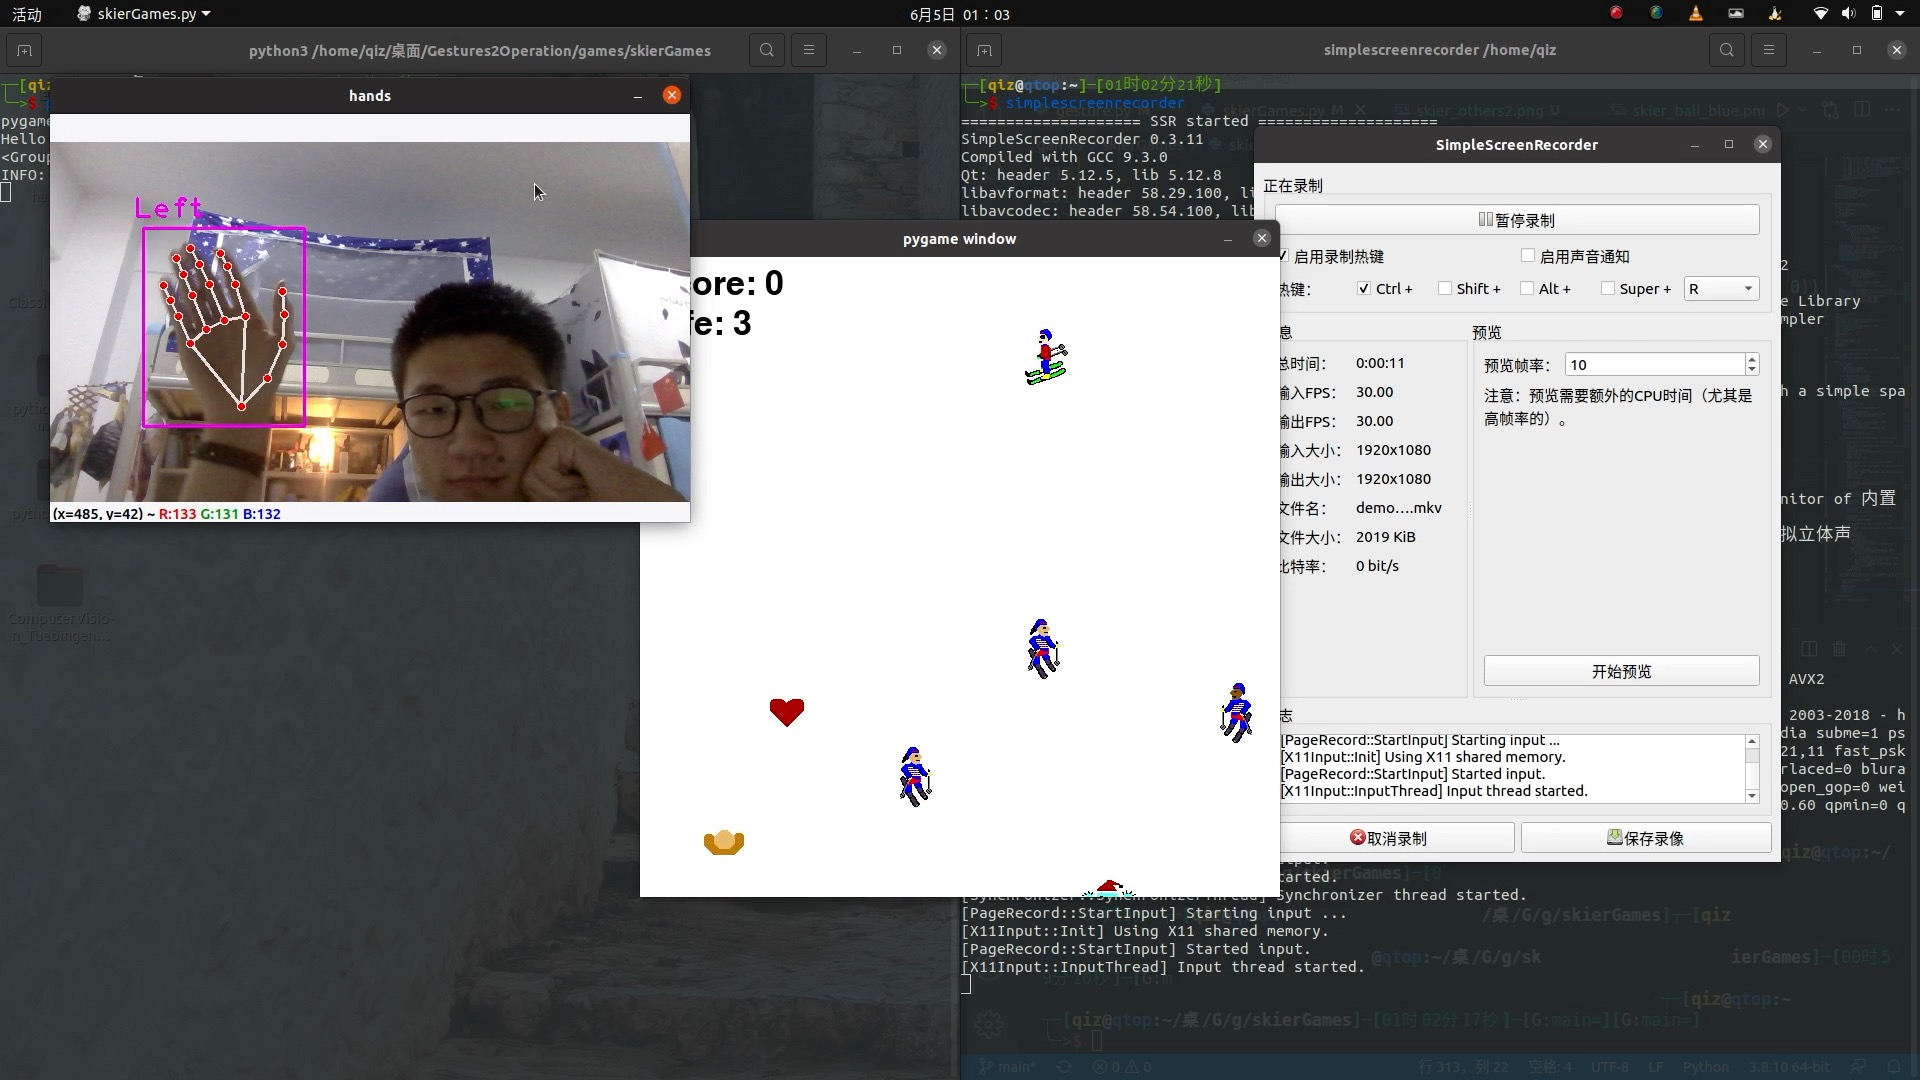
\includegraphics[width=.3\textwidth]{imgs/demo5.jpg}
  \caption{demos\label{pc1}}
\end{figure}

这些demo的运行结果已通过视频的形式上传到了
\href{https://www.bilibili.com/video/BV1tT41157Kq?pop_share=1&vd_source=c567eb8bca008ec5fd0020973414e9c4}
{Bilibili}, 它们各自的细节如下. 

\subsection{虚拟键盘操作}

这个demo的灵感来自于一些科幻电影中的酷炫的虚拟键盘, 如图\ref{vkeyboard}. 
\begin{figure}[htb]
  \centering
  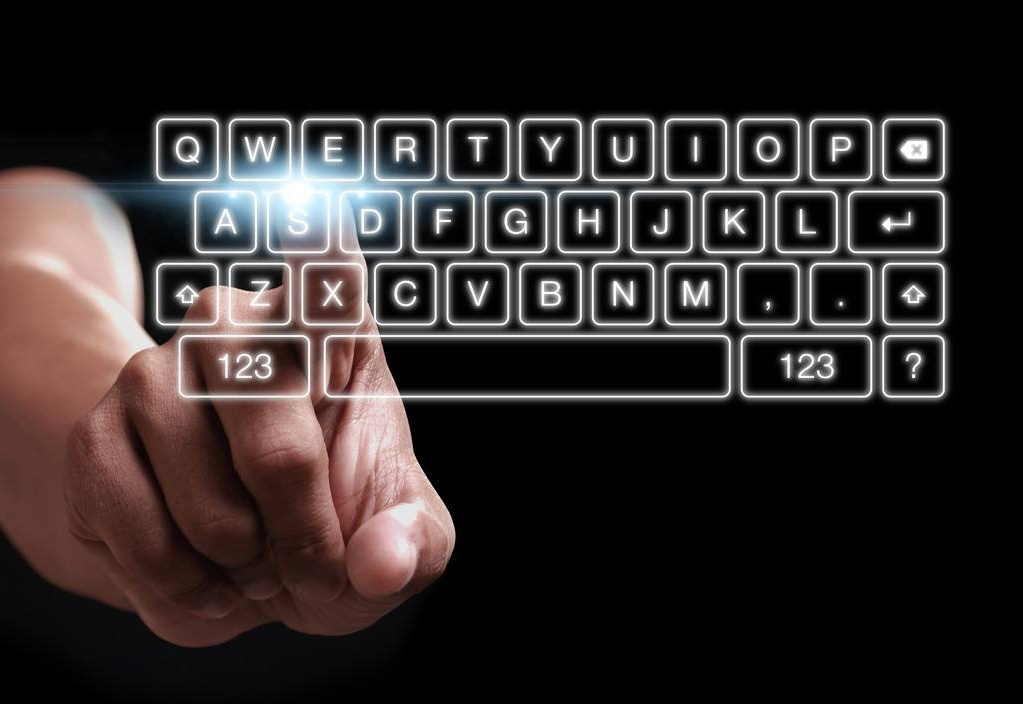
\includegraphics[width=.8\textwidth]{imgs/vkeyboard.jpeg}
  \caption{想象中的虚拟键盘\label{vkeyboard}}
\end{figure}

我们用opencv每一帧地捕捉摄像头的内容, 并将之用mediapipe来扫描, 
最终返回手势内容.
	     
对于键盘,这里用了一个类,将之每个 button封装, 
其内容是位置(pos), 大小(size), 内容(text), 每一帧的图像上都会把它画出来(draw), 
而屏幕上的所有按钮都放在一个列表容器中. 

每次都会检查手指的位置以得到按下来的按钮. 它检查的逻辑是, 
若两个手指, 食指和中指都在一个按钮里面, 就算按下, 同时上一次按下的, 
这一次就无法作为输入(否则会导致一连串输出), 若想输入同一个字母, 则需要先离开当前字母一下.  
并且对于当前按下的键盘, 还设置了相对应的逻辑来符合, 比如shift键和backspace键.

\subsection{在画板上画画}
在画板软件和摄像头就绪的情况下, 需要完成的工作是通过右手食指指尖位置操作鼠标, 
并且要在一些情况完成"光标移动"的操作, 一些情况下完成"光标拖动"的操作. 
Python的pyautogui工具包中提供了moveRel函数用于移动, dragRel函数用于拖动. 
而剩下需要做的事情是识别出用户真正希望做出的操作. 

根据mediapipe包, 可以得到用户当前手势的位置, 但这是存在一定误差的(误差较大), 
对于缓存为$2n$个点的方法, 设$t$时刻计算出指尖的位置为$p(t)$, 将过去$2n$个采样点的
运动近似为匀速直线运动, 这时的速度可被近似为
\[v(t)=\frac{1}{n^2}\sum_{i=0}^{n-1}(p(t-i)-p(t-i-n))\]
这时鼠标要进行的操作就是按照$v(t)$的方向移动或拖动一个正比于$v(t)$长度的距离. 

对于控制移动或拖动, 本文采取的方法为使用左手的大拇指的弯曲与否控制, 而识别左手大拇指
的弯曲程度, 只需要比较大拇指上关键点的折线和直线的差别有多大. 

\subsection{拖动滑块移动}
这个demo的灵感来自于很多国内外科幻电影中存在的虚拟物体交互情节, 如图\ref{block}. 
我们希望仿照它做一个类似的交互, 本文选择的交互对象为虚拟的方块. 
\begin{figure}[htb]
  \centering
  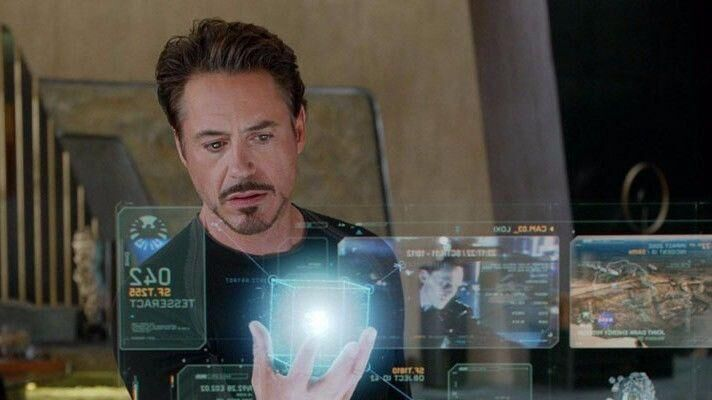
\includegraphics[width=.8\textwidth]{imgs/block.jpg}
  \caption{钢铁侠的非触控交互\label{block}}
\end{figure}

我们的实现方法是每一帧都被摄像头捕捉, 并且检测手指的位置, 对于移动的虚拟物体, 
将之封装成一个类, 每一帧把所有检测物体构成的列表中去对比, 当两个手指比较接近,
\[d_{1} (p_8, p_{12}) \leq C,\] 
则判定为移动状态, 并且实时地把当前被控制物体的中心位置赋值, 若两个手指不够近,
\[d_{1} (p_8, p_{12}) > C,\]
就判断为放下. 并随即更新屏幕内容. 

为了得到更好的体验, 我们还加上了预选则但不提起的加深预览效果.

\subsection{交互网页游戏}
这个demo的灵感来自于有github用户实现了通过广播体操控制2048, 如图\ref{gm4}. 
我们希望将相对不灵活的整个身体改为灵活性较强的手指进行交互, 同时作用于其它基于键盘的游戏. 
\begin{figure}[htb]
  \centering
  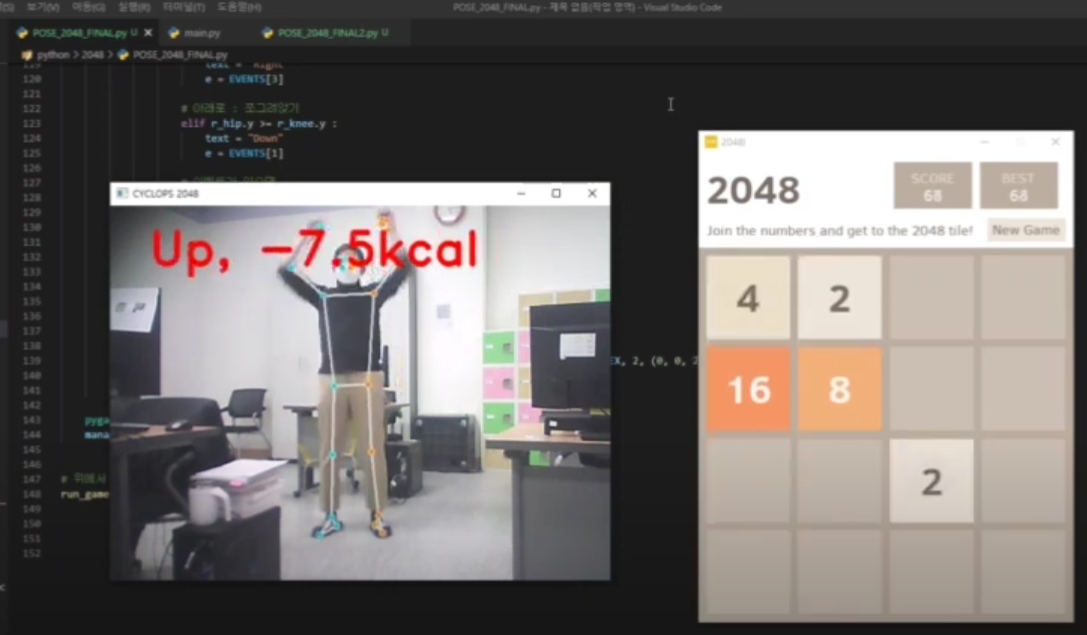
\includegraphics[width=.8\textwidth]{imgs/h2048.png}
  \caption{其它用户实现的交互\label{gm4}}
\end{figure}

部分网页游戏都会要求玩家利用键盘控制游戏进程, 而当这种键盘控制较少的时候, 
就可以利用手势代替键盘输入. 以网页游戏2048为例, 玩家只需要使用上下左右就可操作, 
而使用手势, 可以更自然的做出上下左右的操作. 
Python的pyautogui工具包中提供了press函数用于操作键盘. 
故需要做的事情是识别出用户真正希望做出的操作. 

在第二个demo在画板上画画中, 我们可以计算手的某个位置移动的速度. 
一般地, 当手做出一次向上抬的动作(剩下三个方向同理), 等价于满足手下列三个条件:
\begin{enumerate}
  \item 有一定的向上速度
  \item 比正常位置往上
  \item 上一个时刻不在往上抬
\end{enumerate}

所以只要可以知道正常的位置在哪, 我们就可以计算出手的运动趋势. 
交互过程中, 需要先对手的位置进行校准, 以此的临域作为正常位置, 
再利用上述方法即可完成对网页游戏2048的交互. 
\subsection{交互内置游戏}

这个小项目的灵感来自于Edge浏览器内置的冲浪小游戏, 
比较简约并且有趣, 如图\ref{edge}. 故写了一款内置在Python中的滑雪小游戏, 使用上述
手势方法对它进行操作. 
\begin{figure}[htb]
  \centering
  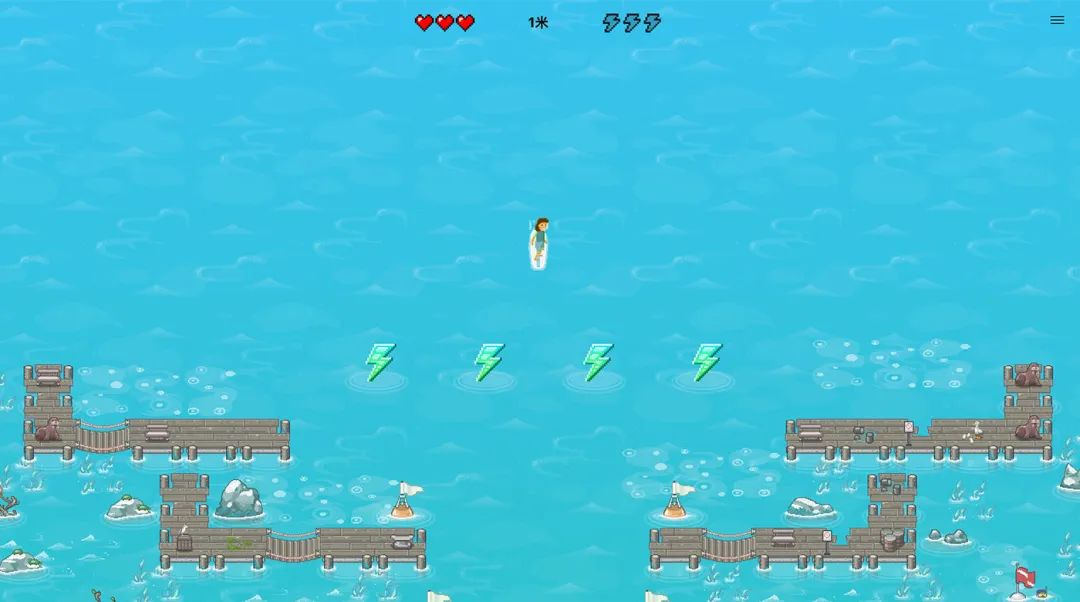
\includegraphics[width=.8\textwidth]{imgs/edge.jpeg}
  \caption{Edge的内置游戏\label{edge}}
\end{figure}

我们把手势识别相关功能封装成了一个类(Gesture\_Monitor),这样就能达到比
较好的代码复用效果, 他方法分别是构建以后, 对每一帧图像更新, 每次更新会带
起检查, 并更新手势的状态, 即当前手势(比如是上,下,左,右等.), 最后可以用
对应的函数查询(is\_left(), is\_right()等), 而在插入游戏的过程中, 我
们只需要把条件放宽就可.
 
本游戏的逻辑是这样的, 地图是由函数随机生成的, 人纵轴不变, 横轴提供交互式. 
障碍物从一开始只有松树对应减分效果,到我们添加到了雪人, 雪怪, 其他玩家, 
几种松树, 对应的buff加成等. 



\section{接下来的工作}

本文的核心方法是基于单张图片去识别动作, 这会使得预测模型的误差被放大. 
我们认为一个可能的改进方法是重新训练一个和时间相关的模型(如循环神经网络), 
对于一段视频进行预测来减少误差; 一个方法是先校准精确位置, 后将检测位置和
经过历史数据进行插值的位置进行加权平均, 作为实际位置. 

当误差被降低到一定范围内, 就可以利用摄像头录制人手骨架运动轨迹, 
从而可以建立3D模型. 这样做出的模型相较于关键帧绘制方法可能会更
符合物理原理, 且成本更低. 


\end{document}
